
%II 
\section{Pré-dimensionnement du Sled $0,3 g$ \label{ccs_mp_2022_sec_2}}
\ifprof
\else
La première étape du développement du Sled $0,3 g$ qui sera utilisé avec des personnes volontaires consiste à prédimensionner certains éléments technologiques pour atteindre les performances définies dans le diagramme des exigences (figure \ref{ccs_mp_2022_fig_A}).

Ainsi, dans une première approche simplifiée, l'ensemble mobile est modélisé par une masse rigide en liaison glissière par rapport au bâti, comme défini sur la figure \ref{ccs_mp_2022_fig_03}. Pour effectuer des campagnes de tests représentatifs du phénomène de coup du lapin avec des personnes volontaires, le profil d'accélération défini sur la figure \ref{ccs_mp_2022_fig_04} est adopté.

\subsubsection*{Modèle cinématique}
\begin{itemize}
  \item Soit $S_{0}$ le bâti lié au sol.
  \item Soit $S$ l'ensemble mobile \{volontaire + siège + plateforme + capteurs\}, en liaison glissière de direction $\vec{x}_{0}$ avec le bâti $S_{0}$.
\end{itemize}

\begin{figure}[!h]
\centering
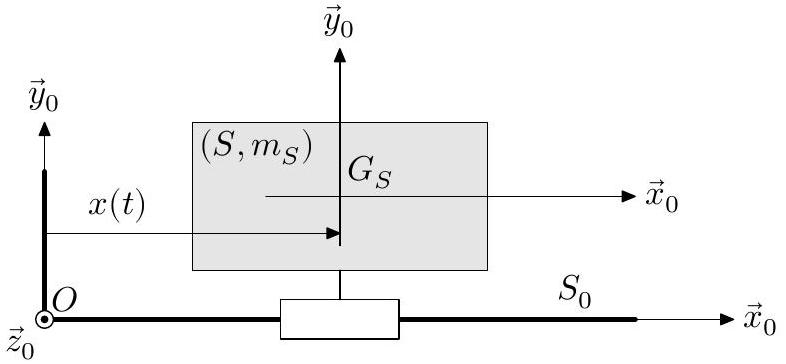
\includegraphics[width=.7\textwidth]{2025_07_06_ec63d2f3afc18cdeeb83g-02}
%Figure 3 
\caption{\label{ccs_mp_2022_fig_03} Modélisation cinématique de l'ensemble mobile $S$ en liaison avec le bâti $S_{0}$}
\end{figure}



\subsubsection*{Notations et données}
\begin{itemize}
  \item Le repère $R_{0}\left(O, \vec{x}_{0}, \vec{y}_{0}, \vec{z}_{0}\right)$ associé au solide $S_{0}$ est supposé galiléen.
  \item Le repère $R_{S}\left(G_{s}, \vec{x}_{0}, \vec{y}_{0}, \vec{z}_{0}\right)$ associé à l'ensemble mobile $S$.
  \item $t$, le temps, exprimé en secondes.
  \item $m_{S}$, la masse de l'ensemble mobile $S, G_{S}$ son centre de gravité tel que $x(t)=\overrightarrow{O G_{S}} \cdot \vec{x}_{0}$.
  \item $\vec{V}_{\left(G_{S}, S / S_{0}\right)}=v(t) \vec{x}_{0}$, la vitesse du centre de gravité $G_{S}$ de l'ensemble mobile $S$ par rapport au bâti $S_{0}$.
  \item $\vec{a}_{\left(G_{S}, S / S_{0}\right)}=a(t) \vec{x}_{0}$, l'accélération du centre de gravité $G_{S}$ de l'ensemble mobile $S$ par rapport au bâti $S_{0}$.
  \item L'accélération de la pesanteur est telle que $\vec{g}=-g \vec{y}_{0}$ avec $g=9,81 \mathrm{~m} \cdot \mathrm{~s}^{-2}$.
\end{itemize}

\subsubsection*{Profil d'accélération type}
\begin{itemize}
  \item L'ensemble mobile $S$ est considéré au repos à l'état initial : ses position, vitesse et accélération sont considérées nulles à l'instant initial.
  \item L'ensemble mobile $S$ est ensuite soumis à un cycle complet d'une accélération constante $a_{c}=+0,3 g$ pendant 1 seconde, puis d'une décélération constante de $-0,3 g$ pendant 1 seconde. Son évolution temporelle, $a(t)$, est présentée sur la figure \ref{ccs_mp_2022_fig_04}.
\end{itemize}

\begin{figure}[!h]
\centering
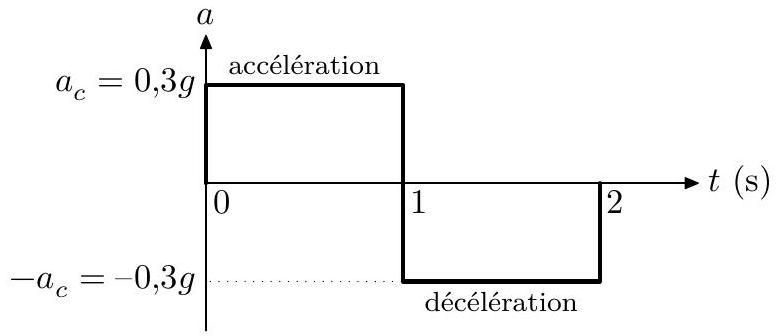
\includegraphics[width=.5\textwidth]{2025_07_06_ec63d2f3afc18cdeeb83g-03}
%Figure 4 
\caption{\label{ccs_mp_2022_fig_04}Évolution de l'accélération au cours du temps}
\end{figure}
%II.A - 
\subsection{Encombrement spatial du Sled 0,3g \label{ccs_mp_2022_sec_2A}}

\begin{obj}
L'objectif est de vérifier que la course du Sled est compatible avec une utilisation dans une salle d'expérimentation.
\end{obj}
\fi


%Q 1. 
\question{\label{ccs_mp_2022_sec_q_01}Déterminer l'expression littérale de la vitesse $v(t)$ en fonction de l'accélération $a_{c}$, dans la première phase d'accélération.}
\ifprof
\begin{corrige}
Lors de la première phase d'accélération on a : $ \dfrac{\text{d}v(t)}{\text{d}t} = a_c \quad \Leftrightarrow \quad \text{d} v(t) = a_c \text{d}t$

D'où : 
$\int_0^t  \text{d} v(t) $ 
$= \int_0^t a_c \text{d}t $
$ = \left[ v(t) \right]_0^t $
$ = \left[ a_c \times t \right]_0^t $
$ = v(t) - v(0) $
$= a_c \times (t - 0) $

Au final, $v(t)  = a_c \times t$.

\end{corrige}
\else
\fi

%Q 2. 
\question{\label{ccs_mp_2022_sec_q_02}En déduire la valeur maximale, notée $V_{\text {max }}$ et exprimée en $\mathrm{m} \cdot \mathrm{s}^{-1}$, de la vitesse atteinte par l'ensemble mobile $S$ au bout d'une seconde avec une accélération constante de $0,3 g$. Conclure sur le respect de l'exigence $\mathrm{Id}=1.1 .2$.}
\ifprof
\begin{corrige}
La fonction $v(t)$ étant continue et croissante, sa valeur maximale est à la fin de la phase d'accélération, soit : $ V_\text{max} = v(1) = a_c \times 1 = 0.3 g \times 1$.

A.N. : $ V_\text{max} = 0.3 \times 9.81 \times 1 = 2.9 \text{ m.s}^{-1} < 3 \text{ m.s}^{-1} \text{  (exigence \texttt{Id 1.1.2})}$.

Donc l'exigence \texttt{Id 1.1.2} est bien respectée.
\end{corrige}
\else
\fi


Un essai complet comprend une phase d'accélération suivie d'une phase de décélération.

%Q 3. 
\question{\label{ccs_mp_2022_sec_q_03}Déterminer la distance maximale théorique, notée $x_{\text {max }}$ et exprimée en m, parcourue par l'ensemble mobile $S$ au cours d'un essai complet. Vérifier le respect de l'exigence Id = 1.2.}
\ifprof
\begin{corrige}
Lors d'un essai complet, il y a une phase d'accélération qui dure une seconde à $\ddot x = a_c$ et une phase de décélération à $\ddot x = - a_c$. On en déduit alors pour chaque phase, les résultats suivants :\\

\begin{minipage}{.5\textwidth}
	\begin{center}Phase d'accélération $\varphi_1$ : pour $t \in [0;1]$\end{center}
$
\begin{array}{l l}
\ddot x_{\varphi_1} & = a_c = 0.3 g\\
\dot x_{\varphi_1} & = v(t) = 0.3 g \times t \rightarrow v(1) = V_\text{max} = 0.3 g \times 1 \\
x_{\varphi_1}(t) & =  0.3 g \times \dfrac{t^2}{2} + x(0) \rightarrow x(1) = \dfrac{0.3}{2} g
\end{array}
$
\end{minipage}
\begin{minipage}{.5\textwidth}
	\begin{center}Phase de décélération $\varphi_2$  : pour $t \in [1;2]$\end{center}
$
\begin{array}{l l}
\ddot x_{\varphi_2} & = -a_c = -0.3 g\\
\dot x_{\varphi_2} & = -0.3 g \times (t-1) + v(1)\\
x_{\varphi_2}(t) & = -0.3 g \times \dfrac{(t-1)^2}{2} + v(1) \times (t-1) + x(1)
\end{array}
$
\end{minipage}

\vspace{1em}
Finalement on a : $x_\text{max} = x_{\varphi_2}(2) = -\dfrac{0.3}{2} g + 0.3 g \times 1 \times 1 + \dfrac{0.3}{2} g$ et $ x_\text{max} = 0.3 g \times 1 \times 1 $.

A.N. $ x_\text{max} = 2.9 \text{ m} < 4.5 \text{ m} \text{  (exigence \texttt{Id 1.2})}$.

Donc l'exigence \texttt{Id 1.2} est bien respectée.
\end{corrige}
\else
\fi

%II.B - 
\subsection{Dimensionnement spatial de l'ensemble mobile \label{ccs_mp_2022_sec_2B}}
%\section*{Objectif}

\begin{obj}
L'objectif est de vérifier la sécurité des passagers et de valider l'emprise au sol du Sled.

Les ingénieurs du bureau d'études envisagent de réaliser la liaison glissière par interposition d'éléments roulants, afin de réduire les pertes énergétiques dans cette liaison et de diminuer également le phénomène d'arc-boutement. Il est à présent nécessaire de vérifier la sécurité des passagers du Sled en étudiant le possible basculement de l'ensemble mobile lors d'un essai.
\end{obj}

\ifprof
\else
\subsubsection*{Hypothèses d'étude}
\begin{itemize}
  \item Pour cette étude, les ingénieurs du bureau d'études choisissent de modéliser la liaison glissière entre l'ensemble mobile $S$ et le bâti $S_{0}$ dans le plan de symétrie ( $O, \vec{x}_{0}, \vec{y}_{0}$ ) de la figure \ref{ccs_mp_2022_fig_05} par deux contacts ponctuels en $A$ et en $B$, de normale $\vec{y}_{0}$, distants de $L$.
  \item L'étude suivante est menée uniquement en phase d'accélération définie pour un essai avec un passager volontaire.
\end{itemize}

\begin{figure}[!h]
\centering
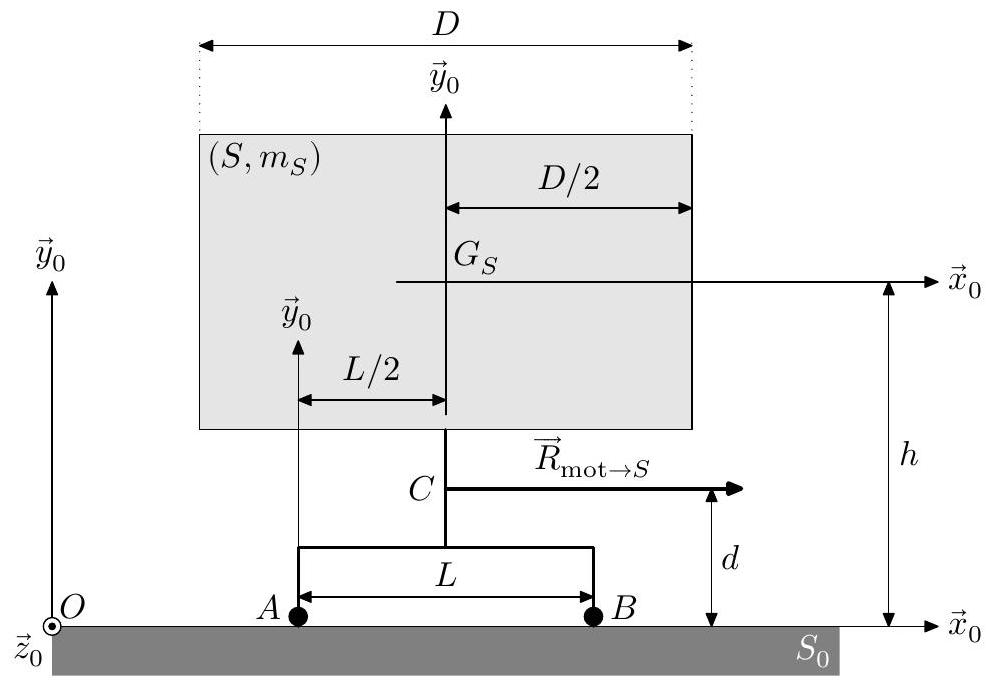
\includegraphics[width=.7\textwidth]{2025_07_06_ec63d2f3afc18cdeeb83g-03(1)}
\caption{\label{ccs_mp_2022_fig_05}Paramétrage de l'ensemble mobile $S$ du Sled}
\end{figure}



\subsubsection*{Notations et données}
\begin{itemize}
  \item Les actions transmissibles par les deux contacts ponctuels seront respectivement notées
\end{itemize}

$$
\left\{T_{A_{S_{0} \rightarrow S}}\right\}=\left\{\begin{array}{c}
Y_{A} \vec{y}_{0} \\
\overrightarrow{0}
\end{array}\right\}_{A} \quad \text { et } \quad\left\{T_{B_{S_{0} \rightarrow S}}\right\}=\left\{\begin{array}{c}
Y_{B} \vec{y}_{0} \\
\overrightarrow{0}
\end{array}\right\}_{B}
$$

\begin{itemize}
  \item L'action mécanique motrice qui permet de mettre en mouvement l'ensemble mobile $S$ par rapport au bâti $S_{0}$ est modélisée par un glisseur au point $C$, noté
\end{itemize}

$$
\left\{T_{\mathrm{mot} \rightarrow S}\right\}=\left\{\begin{array}{c}
\vec{R}_{\mathrm{mot} \rightarrow S}=R \vec{x}_{0} \\
\overrightarrow{0}
\end{array}\right\}_{C}
$$

avec $R>0$ en phase d'accélération.

\begin{itemize}
  \item Les principales caractéristiques dimensionnelles indiquées sur la figure \ref{ccs_mp_2022_fig_05} ont été estimées pour avoir une position réaliste du volontaire dans un siège de voiture, $D=1000 \mathrm{~mm}$, $d=220 \mathrm{~mm}$ et $h=1100 \mathrm{~mm}$.
\end{itemize}
\fi

%II.B.1) 
\subsubsection{Détermination de l'effort normal $Y_{B}$ \label{ccs_mp_2022_sec_2B1}}

%Q 4. 
\question{\label{ccs_mp_2022_sec_q_04}Isoler l'ensemble mobile $S$ et effectuer l'inventaire des actions mécaniques extérieures qui s'appliquent sur cet ensemble.}
\ifprof
\begin{corrige}
On isole $S$, le bilan des actions mécanique à $S$ est :

\begin{itemize}
\item la pesanteur : $\left\{  T_{\text{pes}\to S} \right\} = \begin{Bmatrix} - m_S \, g \, \vec y_0 \\ \overrightarrow{0} \end{Bmatrix}_{G_S}$ 
\item l'action du sol sur $S$ en $A$ : $\left\{  T_{A_{S_0\to S}}\right\} = \begin{Bmatrix} Y_A \, \vec y_0 \\ \overrightarrow{0} \end{Bmatrix}_A $
\item l'action du sol sur $S$ en $B$ :  $\left\{  T_{B_{S_0\to S}}\right\} = \begin{Bmatrix} Y_B \, \vec y_0 \\ \overrightarrow{0} \end{Bmatrix}_B $
\item l'action mécanique motrice : $\left\{ T_{\text{mot}\to S} \right\} = \begin{Bmatrix} \overrightarrow{R}_{\text{mot}\to S} = R \, \vec x_0 \\ \overrightarrow{0} \end{Bmatrix}_C$
\end{itemize}
\end{corrige}
\else
\fi


%Q 5. 
\question{\label{ccs_mp_2022_sec_q_05}Exprimer $\vec{\delta}_{\left(G_{S}, S / S_{0}\right)}$, le moment dynamique en $G_{S}$ de l'ensemble mobile $S$ dans son mouvement par rapport au bâti $S_{0}$. En déduire l'expression littérale du moment dynamique au point $A$ de l'ensemble mobile $S$ dans son mouvement par rapport au bâti $S_{0}$ en fonction de l'accélération $a_{c}$, de la masse $m_{S}$ et d'un paramètre géométrique.}
\ifprof
\begin{corrige}
Le moment dynamique en $G_S$ de l'ensemble $S$ s'exprime comme suit :
$\overrightarrow{\delta}_{G_S, S/S_0} = \left.\dfrac{\text{d} \overrightarrow{\sigma}_{G_S, S/S_0}}{\text{d}t}\right|_{R_0} + m_S \overrightarrow{V}_{G_S} \wedge \overrightarrow{V}_{G_S, S/S_0} = \left.\dfrac{\text{d} \overrightarrow{\sigma}_{G_S, S/S_0}}{\text{d}t}\right|_{R_0} $.

Or :$ \overrightarrow{\sigma}_{G_S, S/S_0} = \overline{\overline{I}}_{G_S, S/S_0} \cdot \overrightarrow{\Omega}_{S/S_0} + m \overrightarrow{G_SG_S} \wedge \overrightarrow{V}_{G_S, S/S_0} = \overline{\overline{I}}_{G_S, S/S_0} \cdot \overrightarrow{\Omega}_{S/S_0}$.

%%La symétrie plane (de plan $(O, \vec x_0, \vec y_0)$) permet de simplifier :
%%
%%\begin{itemize}
%%
%%\item la matrice d'inertie : 
%%$$\overline{\overline{I}}_{G_S, S/S_0} = \begin{pmatrix}  A & -F & {-E}  \\ -F & B & {-D} \\ {-E} & {-D} & C \end{pmatrix}_{G_S, \vec x_0, \vec y_0, \vec z_0}  $$
%%
%%\item le vecteur taux de rotation :
%%$$ \overrightarrow{\Omega}_{S/S_0} = \begin{pmatrix} {\omega_x} \\ {\omega_y} \\ \omega_z \end{pmatrix}_{\vec x_0, \vec y_0, \vec z_0}$$
%%\end{itemize}
%%
%%Le moment cinétique devient alors : $ \overrightarrow{\sigma}_{G_S, S/S_0} = C \, \omega_z \, \vec z_0$
%%
%%Le moment dynamique peut s'écrire : $ \overrightarrow{\delta}_{G_S, S/S_0} = C \dfrac{\text{d}\omega_z}{\text{d}t} \vec z_0$
%
Si on considère qu'on a une liaison glissière de $S/S_0$, alors $\left\{ \mathcal{V}_{S/S_0} \right\} = \begin{Bmatrix} \vec 0 \\ v(t) \vec x_0 \end{Bmatrix}_{G_S}$, donc $\overrightarrow{\Omega}_{S/S_0} = \vec 0$

Donc $\overrightarrow{\sigma}_{G_S, S/S_0} = \vec 0$, d'où :
$ \overrightarrow{\delta}_{G_S, S/S_0} = \vec 0$.


D'après le théorème de Varignon, on a :
$\overrightarrow{\delta}_{A, S/S_0} = \overrightarrow{\delta}_{G_S, S/S_0} + \overrightarrow{AG_S} \wedge m_S \, \overrightarrow{a}_{G_S, S/S_0} $
 $= \vec 0 + \begin{pmatrix}  \dfrac{L}{2} \\ h \\ 0 \end{pmatrix}_{\vec x_0, \vec y_0, \vec z_0} \wedge m_S \begin{pmatrix}  a_c \\ 0 \\ 0 \end{pmatrix}_{\vec x_0, \vec y_0, \vec z_0}$.


Au final, $ \overrightarrow{\delta}_{A, S/S_0} =  - m_S \times h \times a_c \times \vec z_0 $.



\end{corrige}
\else
\fi

%Q 6. 
\question{\label{ccs_mp_2022_sec_q_06}Appliquer le théorème du moment dynamique, à l'ensemble mobile $S$, au point $A$, en projection selon $\vec{z}_{0}$. En déduire l'expression littérale de la composante $Y_{B}$ du contact ponctuel en $B$ en fonction de l'accélération $a_{c}$, de $g$, de la masse $m_{S}$, de paramètres géométriques et de $R$.}
\ifprof
\begin{corrige}
D'après le théorème du moment dynamique appliqué en $A$, en projection sur $\vec z_0$, on a :

$\left( \overrightarrow{\mathcal{M}}_{A, \text{pes} \to S} +  \overrightarrow{\mathcal{M}}_{A, B_{S_0\to S}} + \overrightarrow{\mathcal{M}}_{A, \text{mot} \to S} \right) \cdot \vec z_0 = \overrightarrow{\delta}_{A, S/S_0} \cdot \vec z_0 $.

Il faut donc déplacer les torseurs du bilan des actions mécaniques extérieures en $A$ :

\begin{itemize}
\item $\left\{  T_{\text{pes}\to S} \right\} = \begin{Bmatrix} - m_S \, g \, \vec y_0 \\ \overrightarrow{0} \end{Bmatrix}_{G_S} = \begin{Bmatrix} - m_S \, g \, \vec y_0 \\ \overrightarrow{AG_S} \wedge - m_S \, g \, \vec y_0  = - m_S \times g \times \dfrac{L}{2} \vec z_0 \end{Bmatrix}_{A}  \quad \left(\text{avec : } \overrightarrow{AG_S} = \dfrac{L}{2} \vec x_0 + h \vec y_0 \right)$
\item $\left\{  T_{A_{S_0\to S}}\right\} = \begin{Bmatrix} Y_A \, \vec y_0 \\ \overrightarrow{0} \end{Bmatrix}_A $
\item $\left\{  T_{B_{S_0\to S}}\right\} = \begin{Bmatrix} Y_B \, \vec y_0 \\ \overrightarrow{0} \end{Bmatrix}_B = \begin{Bmatrix} Y_B \, \vec y_0 \\ \overrightarrow{AB} \wedge Y_B \, \vec y_0 = L \times Y_B \vec z_0 \end{Bmatrix}_A \quad \left(\text{avec : } \overrightarrow{AB} = L \vec x_0 \right)$
\item $\left\{ T_{\text{mot}\to S} \right\} = \begin{Bmatrix} R \, \vec x_0 \\ \overrightarrow{0} \end{Bmatrix}_C = \begin{Bmatrix} R \, \vec x_0 \\ \overrightarrow{AC} \wedge R \, \vec x_0 = - d \times R \vec z_0 \end{Bmatrix}_A \quad \left(\text{avec : } \overrightarrow{AC} = \dfrac{L}{2} \vec x_0 + d \vec y_0 \right)$
\end{itemize}

Le théorème du moment dynamique appliqué en $A$ projeté sur $\vec z_0$ s'écrit alors :
$ - m_S \times g \times \dfrac{L}{2} + L \times Y_B - d \times R = - m_S \times h \times a_c $.

Finalement, on obtient l'expression littérale de la composante $Y_B$ :

$ Y_B = \dfrac{m_S \left(g \times \dfrac{L}{2} -\times h \times a_c\right) + d \times R}{L}$
$  = m_S \left( \dfrac{g}{2} - \dfrac{h \times a_c}{L}\right) + \dfrac{d \times R}{L}$.
\end{corrige}
\else
\fi


%II.B.2) 
\subsubsection*{Détermination de la longueur $L$ \label{ccs_mp_2022_sec_2B2}}

%Q 7. 
\question{\label{ccs_mp_2022_sec_q_07}Donner la condition sur $Y_{B}$ qui traduit le non-basculement autour de l'axe ( $A, \vec{z}_{0}$ ) de l'ensemble mobile $S$ lors de la phase d'accélération.}
\ifprof
\begin{corrige}
La condition traduisant le non-basculement est : $ Y_B > 0$.
\end{corrige}
\else
\fi


%Q 8. 
\question{\label{ccs_mp_2022_sec_q_08}Après avoir explicité le système isolé et précisé le théorème utilisé, déterminer l'expression littérale de $R$, en fonction de la masse $m_{S}$ et de l'accélération $a_{c}$.}
\ifprof
\begin{corrige}
On isole l'ensemble mobile $S$ du Sled et on applique le théorème de la résultante dynamique projeté sur l'axe $\vec x_0$ :
$ R = m_S \times \overrightarrow{a}_{G_S, S/S_0} \cdot \vec x_0$ et
$ R = m_S \times a_c$.
\end{corrige}
\else
\fi


%Q 9. 
\question{\label{ccs_mp_2022_sec_q_09}En déduire la longueur minimale du guidage entre l'ensemble mobile $S$ et le bâti $S_{0}$ en fonction de l'accélération $a_{c}$, de $g$ et de paramètres géométriques pour garantir le non-basculement autour de l'axe ( $A, \vec{z}_{0}$ ) lors de la phase d'accélération.}
\ifprof
\begin{corrige}
En prenant en compte la condition de non-basculement et le résultat du théorème de la résultante dynamique appliquée à $S$ en projection sur $\vec x_0$, on obtient :
$  m_S \left( \dfrac{g}{2} - \dfrac{h \times a_c}{L}\right) + \dfrac{d \times m_S \times a_c}{L} > 0$
et $  L > \dfrac{2\,a_c}{g} (h - d)$.

\end{corrige}
\else
\fi


%II.B.3) 
\subsubsection{Validation des exigences associées à la sécurité des passagers et à l'encombrement \label{ccs_mp_2022_sec_2B3}}
%Q 10. 
\question{\label{ccs_mp_2022_sec_q_10}Au regard de l'expression littérale de la longueur minimale du guidage de l'ensemble mobile $S$, indiquer s'il est nécessaire d'adapter cette longueur aux différentes masses de passagers, volontaires ou mannequins.}
\ifprof
\begin{corrige}
La longueur étant indépendante de la masse de l'ensemble isolé $S$, on en déduit qu'il n'est pas nécessaire d'adapter cette longueur $L$ aux différentes masses de passagers, volontaires ou mannequins.
\end{corrige}
\else
\fi


%Q 11. 
\question{\label{ccs_mp_2022_sec_q_11}Déterminer la valeur numérique minimale de la dimension longitudinale $L$ du guidage entre l'ensemble mobile $S$ et le bâti $S_{0}$ afin de garantir le respect de l'exigence Id $=1.3$ lors de la phase d'accélération définie.}
\ifprof
\begin{corrige}
L'exigence \texttt{Id = 1.3} de non-basculement donne que la dimension longitudinale minimale est :
$ L_\text{min} = \dfrac{2\,a_c}{g} (h - d) = \dfrac{2\times 0.3 g}{g} (h - d)$.

A.N. :$ L_\text{min} = 2 \times 0.3 \times (1100 - 220) = 528 \text{ mm}$.
\end{corrige}
\else
\fi


%Q 12. 
\question{\label{ccs_mp_2022_sec_q_12}Conclure quant au respect de l'exigence $\mathrm{Id}=1.2$.}
\ifprof
\begin{corrige}
L'exigence \texttt{Id = 1.2} impose une dimension maximale du Sled de $4.5$ m. 

Or la dimension du Sled est $X+L_\text{min}$ d'où l'application numérique :
$ X + L_\text{min} = 2.9 + 0.528 = 3.428 \text{ m} < 4.5 \text{ m}$. 
L'exigence \texttt{Id = 1.2} est donc bien respectée.
\end{corrige}
\else
\fi

\ifprof
\else

\ifprof
\else
Cette étude a conduit les ingénieurs à concevoir une solution pour la liaison glissière mettant en œuvre des galets positionnés au-dessus et en dessous d'un rail (figure \ref{ccs_mp_2022_fig_06}). Des systèmes de réglages sont prévus pour garantir le contact bilatéral et ainsi réduire le risque possible de basculement de l'ensemble mobile $S$.\\
\fi

\begin{figure}[!h]
\centering
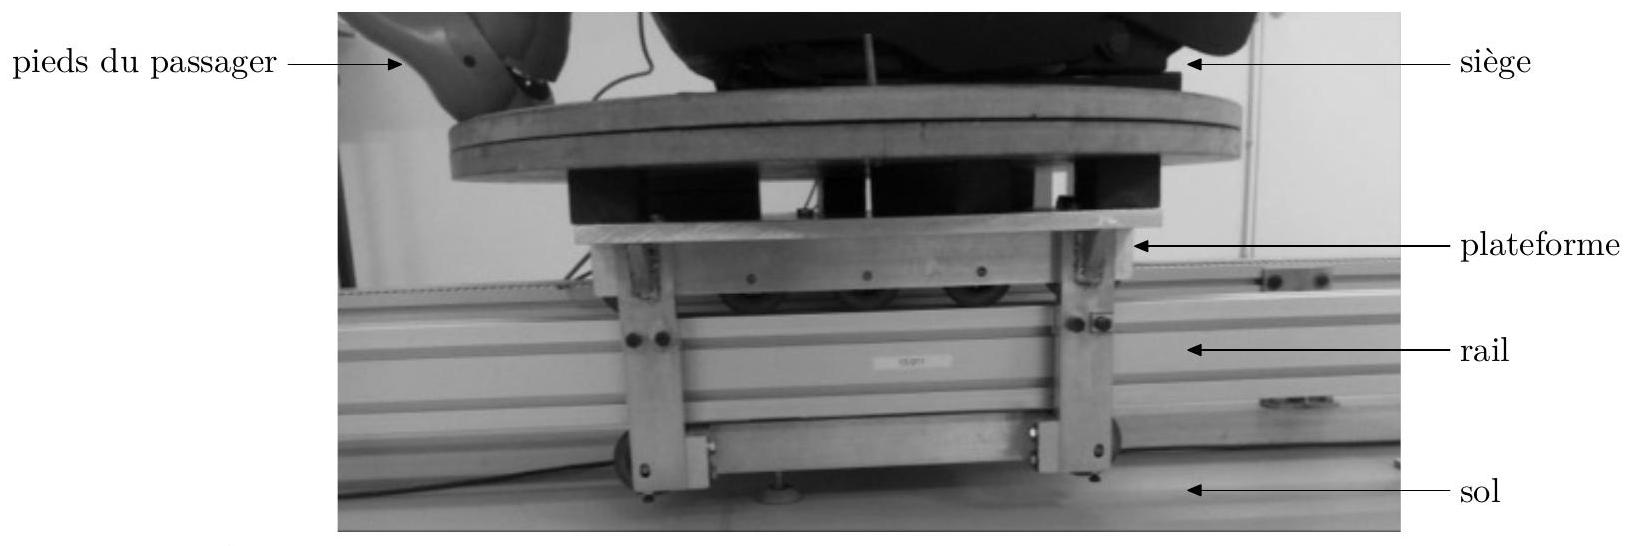
\includegraphics[width=\textwidth]{2025_07_06_ec63d2f3afc18cdeeb83g-04}

%Figure 6 
\caption{\label{ccs_mp_2022_fig_06}Solution retenue pour la réalisation de la liaison glissière entre l'ensemble mobile et le bâti}
\end{figure}
\fi
